% Validation pyramid — 6 automated layers (cheap base → expensive apex)
% with layer 7 (domain correctness, human-only) floating above the stack.
%
% Implementation note: rectangles with decreasing widths centered on x=0
% give the pyramid silhouette without trapezium-positioning quirks.
% Bottom = widest = cheapest. Apex = narrowest = most expensive (still
% automatable). Layer 7 sits separately above with a vertical gap to
% emphasize it's outside the automated stack.
\documentclass[tikz,border=4mm]{standalone}
\usepackage{tikz}
\usetikzlibrary{positioning, arrows.meta}

\begin{document}
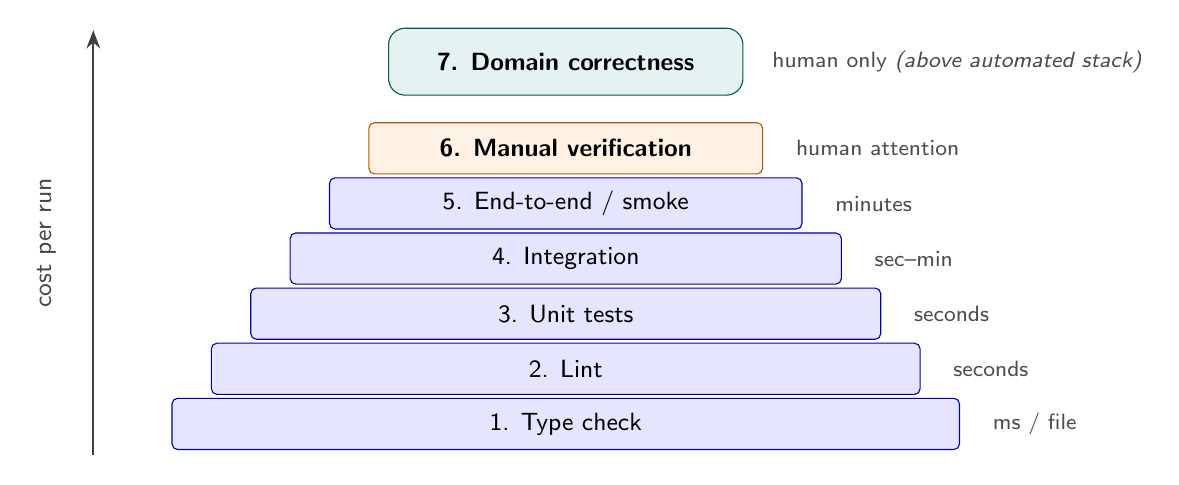
\begin{tikzpicture}[
  font=\sffamily,
  layer/.style={
    draw=blue!70!black, fill=blue!10,
    minimum height=0.65cm, align=center, font=\sffamily\small,
    rounded corners=2pt
  },
  apex/.style={layer,
    draw=orange!70!black, fill=orange!10,
    font=\sffamily\small\bfseries
  },
  human/.style={
    draw=teal!70!black, fill=teal!10,
    minimum height=0.85cm, align=center, font=\sffamily\small\bfseries,
    rounded corners=6pt
  },
  cost/.style={font=\sffamily\footnotesize, text=gray!60!black},
  axislabel/.style={font=\sffamily\small, text=gray!55!black},
]

% Layers centered on x=0 with decreasing widths (pyramid silhouette)
\node[layer, minimum width=10cm] (l1) at (0, 0)    {1. Type check};
\node[layer, minimum width=9cm]  (l2) at (0, 0.7)  {2. Lint};
\node[layer, minimum width=8cm]  (l3) at (0, 1.4)  {3. Unit tests};
\node[layer, minimum width=7cm]  (l4) at (0, 2.1)  {4. Integration};
\node[layer, minimum width=6cm]  (l5) at (0, 2.8)  {5. End-to-end / smoke};
\node[apex,  minimum width=5cm]  (l6) at (0, 3.5)  {6. Manual verification};

% Layer 7 — separated, human-only
\node[human, minimum width=4.5cm] (l7) at (0, 4.6) {7. Domain correctness};

% Cost annotations on the right, indented inward to follow the pyramid edge
\node[cost, anchor=west] at (5.3, 0)   {ms / file};
\node[cost, anchor=west] at (4.8, 0.7) {seconds};
\node[cost, anchor=west] at (4.3, 1.4) {seconds};
\node[cost, anchor=west] at (3.8, 2.1) {sec–min};
\node[cost, anchor=west] at (3.3, 2.8) {minutes};
\node[cost, anchor=west] at (2.8, 3.5) {human attention};
\node[cost, anchor=west] at (2.5, 4.6) {human only \emph{(above automated stack)}};

% Vertical "cost per run" axis on the left
\draw[-Stealth, thick, draw=gray!50!black] (-6, -0.4) -- (-6, 5.0);
\node[axislabel, rotate=90, anchor=south] at (-6.35, 2.3) {cost per run};

\end{tikzpicture}
\end{document}
